% !TEX program = xelatex
% !TeX TXS-program:compile = txs:///xelatex/[-shell-escape]
\documentclass[x11names,svgnames, usepdftitle=false]{beamer}

\usetheme{metropolis}
\setbeamertemplate{caption}{\raggedright\insertcaption\par}
\setbeamercolor{block title}{fg=LightSkyBlue4}
\usepackage{fontspec}
\usepackage{textcomp}
\usepackage{minted}
\usepackage{qrcode}
\usepackage[francais]{babel}
\providecommand{\og}{«\,}
\providecommand{\fg}{\,»}
\usepackage{xspace}
\usepackage[normalem]{ulem}
\usepackage{amsmath}
\usepackage{pifont}
\usepackage{marvosym}
\usepackage{tikz}
\usetikzlibrary{calc, positioning, arrows, shapes, decorations.pathmorphing}

% ------------------------------------------------------------------
% Couleurs : celles du support d'origine (bleu clair, jaune, vert d'eau, orange)
% + code couleur du cours : indice / position = bleu, élément / valeur = rouge
% ------------------------------------------------------------------
\definecolor{cmblue}{RGB}{86, 185, 238}
\definecolor{cmgold}{RGB}{244, 197, 66}
\definecolor{cmmint}{RGB}{224, 245, 240}
\definecolor{cmpeach}{RGB}{250, 215, 180}
\definecolor{cmred}{RGB}{232, 64, 32}
\definecolor{minibar}{RGB}{35, 55, 59}
\colorlet{idxcol}{blue!60!black}% indice / position
\colorlet{eltcol}{red!70!black}% élément / valeur d'une case

% ------------------------------------------------------------------
% Macros pour dessiner une liste (rangée de 8 cases de 1,3 cm)
% ------------------------------------------------------------------
% la rangée : #1,#2 = coin haut gauche
\newcommand{\rangee}[2]{%
  \draw[very thick, rounded corners=3pt] (#1,#2) rectangle ({#1+10.4},{#2-0.9});
  \foreach \i in {1,...,7}{\draw[thick] ({#1+1.3*\i},#2) -- ({#1+1.3*\i},{#2-0.9});}%
}
% contenu d'une case : #1,#2 = coin haut gauche de la rangée, #3 = numéro de case, #4 = élément
\newcommand{\caseval}[4]{\node[font=\ttfamily\scriptsize, text=eltcol] at ({#1+1.3*(#3)+0.65},{#2-0.45}) {#4};}
% indice sous une case
\newcommand{\caseidx}[3]{\node[font=\Large\bfseries, text=idxcol] at ({#1+1.3*(#3)+0.65},{#2-1.35}) {#3};}
% étiquette encadrée en jaune
\newcommand{\boite}[3]{\node[anchor=west, draw=cmgold, rounded corners=5pt, very thick, inner sep=5pt, font=\large] at (#1,#2) {#3};}
% puce : tiret bleu
\newcommand{\tiret}{\textcolor{cmblue}{\rule[0.35ex]{0.8em}{0.4ex}}\hspace{0.5em}}
% bulle (algorithme classique) : #1 = couleur, #2,#3 = centre, #4 = largeur, #5 = texte
\newcommand{\bulle}[5]{%
  \node[fill=#1, rounded corners=14pt, minimum width=#4cm, minimum height=0.9cm, text width={#4cm-0.3cm}, text=black!45, font=\scriptsize\bfseries, align=center] at (#2,#3) {#5};%
}

\hypersetup{
  colorlinks,
  allcolors=.,
  urlcolor=DarkBlue,
  pdftitle=Algorithmique et Programmation 1 - CM5
}

\author{}
\date{Lundi 12 octobre 2026}

\title{
\includegraphics[width=0.75\textwidth]{img/logo-igm.png} \\[1em] Algorithmique et Programmation 1}
\subtitle{CM5 : les listes}
\institute{L1 Mathématiques - L1 Informatique \\ Semestre 1}

\begin{document}

\maketitle

% ==================================================================
% Wooclap
% ==================================================================
\begin{frame}{Le Wooclap}
  \begin{columns}[c]
    \begin{column}{0.40\textwidth}
      \centering
      \qrcode[height=3.8cm]{https://app.wooclap.com/NYURBT}
      \par\smallskip
      {\scriptsize\href{https://app.wooclap.com/NYURBT}{Copier le lien de participation}}
    \end{column}
    \begin{column}{0.58\textwidth}
      \begin{enumerate}
        \item Allez sur \textbf{wooclap.com}
        \item Entrez le code d'événement dans le bandeau supérieur
      \end{enumerate}
      \bigskip
      \begin{center}
        \small Code d'événement\\[0.4em]
        {\Huge\bfseries\color{cmblue} NYURBT}
      \end{center}
      \medskip
      {\scriptsize\itshape Activer les réponses par SMS}
    \end{column}
  \end{columns}
\end{frame}

% ==================================================================
% Dans l'épisode précédent (rappel de deux slides du CM4)
% ==================================================================
\begin{frame}{Dans l'épisode précédent\dots}
  \centering
  \only<2>{%
    \begin{tikzpicture}[scale=0.82, transform shape]
      \fill[black!4] (-5.5,-3.6) rectangle (5.5,3.9);
      \fill[minibar] (-5.5,3.9) rectangle (5.5,4.9);
      \node[anchor=west, text=white] at (-5.3,4.4) {Anatomie d'une fonction};
      \node [draw, rectangle, text width=2cm, minimum height=1.5cm, align=center] (function) at (0,0) {Fonction};
      \draw[-latex] (-5,0) -- (-1.2,0) node[midway, above, label={below: (paramètres)}] {Entrée};
      \draw[-latex] (1.2,0) -- (5,0) node[midway, above, label={below: (valeur de retour)}] {Sortie};
      \draw[decorate, -latex, decoration={snake, segment length=5mm, amplitude=1mm, post length=1mm}] (0,0.75) -- (0,3) node[midway, left] {Affichages};
      \draw[decorate, -latex, decoration={snake, segment length=5mm, amplitude=1mm, post length=1mm}] (0,-0.75) -- (0,-3) node[midway, left] {Effets de bord} node[midway, right] {(aka : Effets secondaires)};
    \end{tikzpicture}%
  }%
  \only<3>{%
    \begin{tikzpicture}
      \fill[black!4] (0,0) rectangle (9.8,-4.9);
      \fill[minibar] (0,0) rectangle (9.8,0.9);
      \node[anchor=west, text=white] at (0.3,0.45) {Pile d'appels};
      \node[anchor=north west, text width=9.3cm, align=left, font=\small] at (0.3,-0.2) {%
        {\color{LightSkyBlue4}Quand un nouvel appel commence}
        \begin{itemize}\setlength{\itemsep}{0pt}
          \item l'exécution de la fonction en cours s'interrompt
          \item un nouvel espace de noms local est créé
          \item l'exécution de la fonction appelée commence
        \end{itemize}
        {\color{LightSkyBlue4}Quand l'appel en cours se termine}
        \begin{itemize}\setlength{\itemsep}{0pt}
          \item son espace de nom est supprimé de la pile
          \item l'exécution de l'appel précédent reprend
        \end{itemize}};
    \end{tikzpicture}%
  }%
\end{frame}

% ==================================================================
% Appels imbriqués
% ==================================================================
\begin{frame}{Appels imbriqués - une allégorie}
  \centering
  \only<1-2>{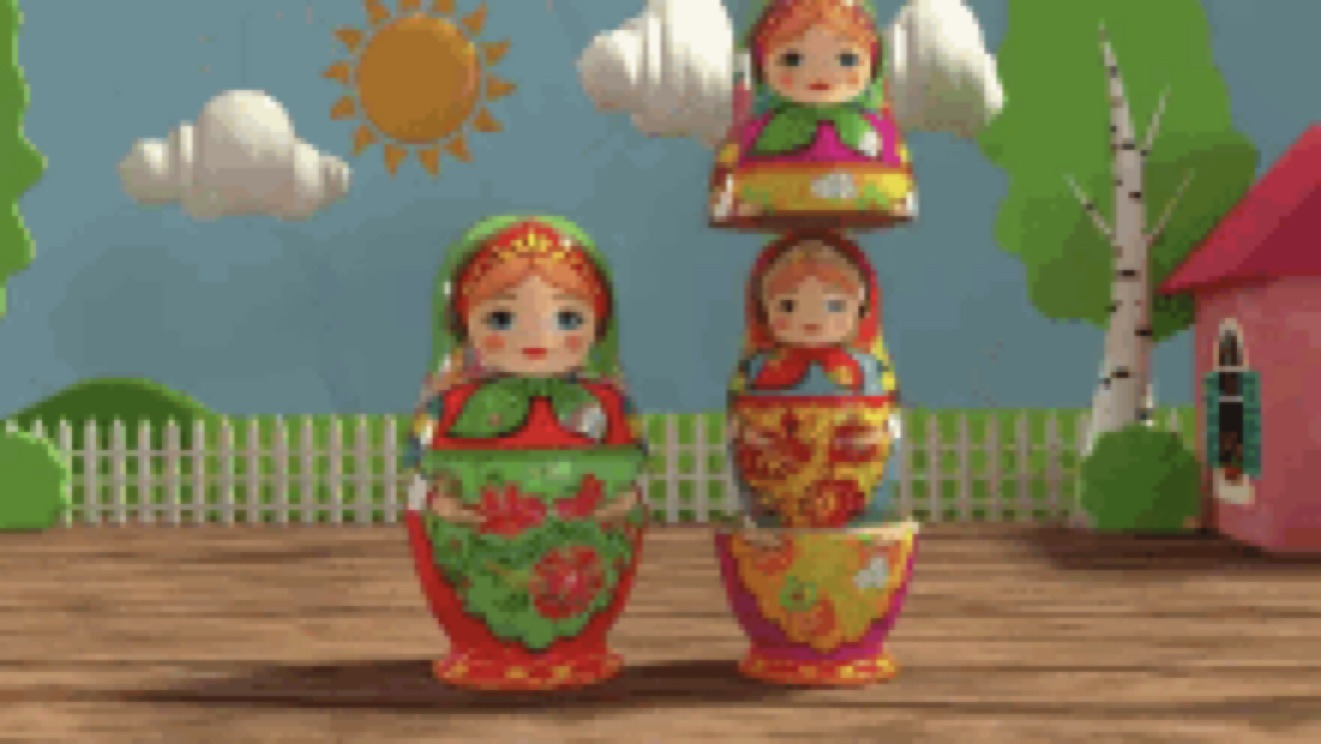
\includegraphics[width=0.85\textwidth]{img/poupees.jpg}}%
\end{frame}

\begin{frame}[fragile]{Appels imbriqués - exemple}
  \begin{columns}[T]
    \begin{column}{0.2\textwidth}
      
\includegraphics[width=\linewidth]{img/matriochka.png}
    \end{column}
    \begin{column}{0.47\textwidth}
\begin{minted}[bgcolor=cmmint, fontsize=\fontsize{6}{6.6}\selectfont]{python}
def f(phrase):
    phrase = phrase + "petite "
    return g(h(phrase))

def g(phrase):
    phrase = phrase + "brise "
    return h(phrase)

def h(phrase):
    if phrase[0] == "L":
        phrase = phrase + "la "
        return k(phrase)
    else :
        return "La " + phrase

def k(phrase):
    return phrase + "glace."

phrase_test = ""
phrase_test = f(phrase_test)
\end{minted}
    \end{column}
    \begin{column}{0.27\textwidth}
      \begin{tikzpicture}
        \node[fill=cmmint, rounded corners=14pt, text width=2.4cm, minimum height=5.2cm, align=center, text=black!40, font=\footnotesize\bfseries] {ILLUSTRATION DU COMPORTEMENT EN MÉMOIRE SUR PYTHON \href{https://pythontutor.com/}{\underline{TUTOR}}};
      \end{tikzpicture}
    \end{column}
  \end{columns}
\end{frame}

% ==================================================================
% Les listes
% ==================================================================
\begin{frame}
  \centering
  \vfill
  {\fontsize{40}{44}\selectfont\bfseries\color{cmblue} Les listes~!!!}
  \vfill
\end{frame}

\begin{frame}{Les listes}
  \begin{tikzpicture}[x=1cm,y=1cm]
    \useasboundingbox (0,0) rectangle (10.6,6.2);

    % --- en haut à droite ---
    \only<2->{\node[anchor=east, font=\itshape\large, text=black!65] at (10.5,5.8) {$\sim$~Tableaux};}

    % --- l'instruction en cours (à gauche) ---
    \only<3-4>{\node[anchor=west, font=\ttfamily\large] at (0.2,5.0) {lst =};}
    \only<5-8>{\node[anchor=west, font=\ttfamily\large] at (0.2,5.0) {lst = ['coucou', 'les', 'AP1']};}
    \only<9->{\node[anchor=west, font=\ttfamily\large] at (0.2,5.0) {lst[2] = 'gens'};}

    % --- « liste ← » et le contenu en petit (à droite) ---
    \only<3->{\node[anchor=east, font=\itshape\large, text=black!65] at (10.5,5.0) {liste $\leftarrow$};}
    \only<6->{\node[anchor=east, font=\ttfamily\tiny, text=black!65] at (10.5,4.65) {['coucou', 'les', 'AP1']};}

    % --- la rangée de cases ---
    \only<2-3,5-7,9-21>{\rangee{0.1}{4.25}}
    \only<6-7,9-21>{\caseval{0.1}{4.25}{0}{'coucou'}\caseval{0.1}{4.25}{1}{'les'}}
    \only<6-7,9>{\caseval{0.1}{4.25}{2}{'AP1'}}
    \only<10-21>{\caseval{0.1}{4.25}{2}{'gens'}}
    \only<13,15,16,18,20>{\caseval{0.1}{4.25}{3}{'!!!'}}
    \only<7,9-21>{\caseidx{0.1}{4.25}{0}\caseidx{0.1}{4.25}{1}\caseidx{0.1}{4.25}{2}}
    \only<13,15,16,18,20>{\caseidx{0.1}{4.25}{3}}

    % --- le meuble à tiroirs (la liste) ---
    \only<4,8>{%
      \node[anchor=north, inner sep=0pt] (commode) at (5.3,5.15) {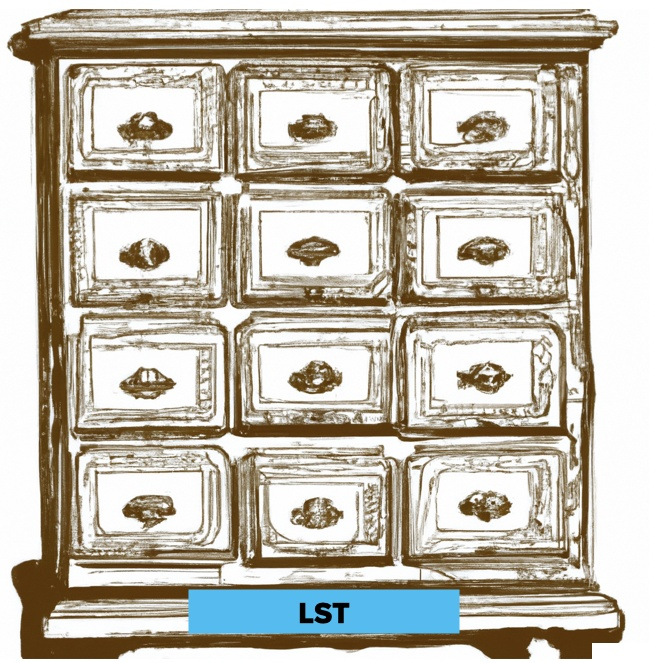
\includegraphics[height=4.5cm]{img/commode.jpg}};
      \node[fill=cmblue, minimum width=1.83cm, minimum height=0.31cm, font=\scriptsize\bfseries, inner sep=0pt]
        at ($(commode.north west)+(0.49*4.5*0.995,-0.92*4.5)$) {LST};
    }
    \only<8>{%
      \foreach \j/\px in {0/0.218, 1/0.480, 2/0.744}{
        \node[fill=cmgold, minimum width=0.19cm, minimum height=0.33cm, font=\scriptsize\bfseries, inner sep=0pt]
          at ($(commode.north west)+({\px*4.5*0.995},{-0.173*4.5})$) {\j};
      }
    }

    % --- instructions sur les listes (en bas) ---
    \only<11-17>{\node[anchor=west, font=\ttfamily] at (0.2,2.2) {lst.append('!!!')};}
    \only<14-17>{\node[anchor=east, font=\itshape\footnotesize, text=black!70] at (10.5,2.2) {Ajouter ‘!!!’ à (la fin de) liste};}
    \only<16-17>{\node[anchor=west, font=\ttfamily] at (0.2,1.6) {lst.pop()};
                 \node[anchor=east, font=\itshape\footnotesize, text=black!70] at (10.5,1.6) {Extraire le (dernier) élément de liste};}
    \only<18-19>{\node[anchor=west, font=\ttfamily] at (0.2,2.2) {lst.extend(lst2)};
                 \node[anchor=east, font=\itshape\footnotesize, text=black!70] at (10.5,2.2) {Ajouter les éléments de lst2 à (la fin de) liste};
                 \node[anchor=west, font=\ttfamily] at (0.2,1.6) {lst.index(elm)};
                 \node[anchor=east, font=\itshape\footnotesize, text=black!70] at (10.5,1.6) {Renvoyer le (premier) indice où se trouve elm};}
    \only<20-21>{\node[anchor=west, font=\Large, text=cmblue] at (0.2,2.0) {Plus :};
                 \node[anchor=west, font=\scriptsize\bfseries, align=left] at (1.6,2.0) {\href{https://docs.python.org/fr/3/library/stdtypes.html\#sequence-types-list-tuple-range}{\underline{https://docs.python.org/fr/3/library/stdtypes.html}}\\ \href{https://docs.python.org/fr/3/library/stdtypes.html\#sequence-types-list-tuple-range}{\underline{\#sequence-types-list-tuple-range}}};}
  \end{tikzpicture}
\end{frame}

\begin{frame}
  \centering
  \vfill
  {\fontsize{30}{34}\selectfont\bfseries\itshape\color{cmblue} Les utiliser, les parcourir\dots.}
  \vfill
\end{frame}

\begin{frame}{Les listes}
  \begin{tikzpicture}[x=1cm,y=1cm]
    \useasboundingbox (0,0) rectangle (10.6,6.2);

    \node[anchor=east, font=\bfseries\itshape\large, text=cmblue] at (10.5,5.85) {Les utiliser, les parcourir\dots.};

    % --- la liste, avec ses indices ---
    \rangee{0.1}{5.35}
    \caseval{0.1}{5.35}{0}{'coucou'}\caseval{0.1}{5.35}{1}{'les'}\caseval{0.1}{5.35}{2}{'gens'}\caseval{0.1}{5.35}{3}{'!!!'}
    \caseidx{0.1}{5.35}{0}\caseidx{0.1}{5.35}{1}\caseidx{0.1}{5.35}{2}\caseidx{0.1}{5.35}{3}

    % --- en général : de gauche à droite, case par case ---
    \only<1-3>{\node[anchor=west, font=\large] (eg) at (0.2,3.3) {\textcolor{cmblue}{\bfseries En général :} de gauche à droite,~};}
    \only<1>{\node[anchor=west, font=\large, inner sep=5pt] at (eg.east) {case par case};}
    \only<2-3>{\node[anchor=west, font=\large, draw=cmgold, rounded corners=5pt, very thick, inner sep=5pt] at (eg.east) {case par case};}
    \only<3>{\node[font=\large] at (5.3,2.5) {Élément par élément};
             \node[font=\bfseries, text=cmblue] at (5.3,1.85) {OU};
             \node[font=\large] at (5.3,1.2) {Indice par indice};}

    % --- élément par élément ---
    \only<4-5>{\boite{0.1}{3.3}{Élément par élément :}
               \node[anchor=north west, align=left, font=\Large] at (0.25,2.6) {\textbf{for} elem \textbf{in} liste :\\[2pt] \hspace{0.6cm}$\mid$ instructions};}
    \only<5>{\node[anchor=north west, align=left, font=\small\itshape, text=black!55] at (5.6,2.35) {\textbf{Pour chaque} élément \textbf{de} liste :\\ \hspace{0.4cm}$\mid$ instructions};}

    % --- indice par indice ---
    \only<6-9>{\boite{0.1}{3.3}{Indice par indice :}
               \node[anchor=north west, align=left, font=\large] at (0.25,2.65) {indice = 0\\[1pt] \textbf{while} indice < len(liste) :\\[1pt] \hspace{0.5cm}$\mid$ instructions\\[1pt] \hspace{0.5cm}$\mid$ \dots.\\[1pt] \hspace{0.5cm}$\mid$ indice += 1};}
    \only<7-9>{\node[font=\Huge\bfseries, text=cmblue] at (5.7,1.7) {OU};}
    \only<8-9>{\node[anchor=north west, align=left, font=\normalsize] at (6.6,2.45) {\textbf{for} indice \textbf{in}\\ range(len(liste)) :\\ \hspace{0.5cm}$\mid$ instructions};}
    \only<9>{\node[anchor=north west, align=left, font=\small\itshape, text=black!55] at (6.6,0.95) {\textbf{Pour} i \textbf{allant de} 0 \textbf{à} n :\\ \hspace{0.4cm}instructions};}

    % --- les deux ---
    \only<10-15>{\boite{0.1}{3.3}{Les deux :}}
    \only<10>{\node[anchor=north west, align=left, font=\large] at (0.2,2.55) {\textbf{for} i, elt \textbf{in} \textbf{enumerate}(liste) :\\[2pt] \hspace{0.6cm}$\mid$ instructions};}
    \only<11-15>{\node[anchor=north west, align=left, font=\large] at (0.2,2.55) {\textbf{for} i, elt \textbf{in} \textbf{enumerate}(liste) :\\[2pt] \hspace{0.6cm}$\mid$ print(i, elt)};}
    \only<12->{\node[font=\Large\bfseries, text=idxcol] at (7.4,3.3) {0};\node[font=\ttfamily\small, text=eltcol] at (8.9,3.3) {'coucou'};}
    \only<13->{\node[font=\Large\bfseries, text=idxcol] at (7.4,2.65) {1};\node[font=\ttfamily\small, text=eltcol] at (8.9,2.65) {'les'};}
    \only<14->{\node[font=\Large\bfseries, text=idxcol] at (7.4,2.0) {2};\node[font=\ttfamily\small, text=eltcol] at (8.9,2.0) {'gens'};}
    \only<15->{\node[font=\Large\bfseries, text=idxcol] at (7.4,1.35) {3};\node[font=\ttfamily\small, text=eltcol] at (8.9,1.35) {'!!!'};}
  \end{tikzpicture}
\end{frame}

% ==================================================================
% Parcours : élément par élément ou indice par indice, pour tous les itérables
% ==================================================================
\begin{frame}
  \begin{tikzpicture}[x=1cm,y=1cm]
    \useasboundingbox (0,0) rectangle (10.6,6.6);
    \node[align=center, font=\LARGE] at (5.3,5.9) {\textcolor{cmblue}{\bfseries En général :} \textcolor{cmblue}{parcours} de gauche à droite};
    \node[font=\LARGE] at (3.7,4.9) {Élément par élément};
    \node[font=\large\bfseries, text=cmblue] at (3.7,4.1) {OU};
    \node[font=\LARGE] at (3.7,3.3) {Indice par indice};
    \only<2->{\node[fill=cmblue, font=\Large\bfseries, text=black, inner sep=4pt] at (5.3,1.7) {SEULEMENT POUR LES LISTES ???};}
    \only<3->{\node[fill=cmblue, font=\Large\bfseries, text=black, inner sep=4pt] at (5.3,0.8) {NON : \og ITERABLES \fg};}
    \only<4>{%
      \node[fill=cmmint, rounded corners=14pt, anchor=north east, text width=2.5cm, inner sep=8pt, font=\small, text=black!70] at (10.5,5.4) {%
        \tiret Listes\\[2pt] \tiret Chaînes\\[2pt] \tiret \textit{Tuples}\\[2pt] \tiret \textit{Ensembles}\\[2pt] \tiret \textit{Fichiers\dots}};}
  \end{tikzpicture}
\end{frame}

% ==================================================================
% Revenons aux listes : les algorithmes classiques
% ==================================================================
\begin{frame}{Revenons aux listes}
  \begin{tikzpicture}[x=1cm,y=1cm]
    \useasboundingbox (0,0) rectangle (10.6,6.2);

    \only<1-5>{%
      \node[anchor=west, font=\footnotesize\bfseries, text=black!70] at (0.2,5.6) {\tiret Algorithmes classiques sur les listes :};
      \node[anchor=west, font=\footnotesize\bfseries, text=black!70] at (0.6,4.7) {\tiret Parcours pour :};
      \node[anchor=west, font=\footnotesize\bfseries, text=black!70] at (1.0,3.8) {\tiret Trouver un élément ou un indice};
      \node[anchor=west, font=\footnotesize\bfseries, text=black!70] at (1.0,3.0) {\tiret Etablir une propriété};
    }
    \only<5>{%
      \node[anchor=west, font=\footnotesize\bfseries, text=black!70, align=left] at (1.0,1.9) {\tiret Calculer une quantité,\\ \hspace{1.3em}fabriquer une liste};
      \node[anchor=west, font=\footnotesize\bfseries, text=black!70] at (0.6,0.8) {\tiret \textit{Plus tard :} \textit{Modifier} la liste};
    }

    % --- les bulles, qui s'ajoutent ---
    \only<2-5>{\bulle{cmmint}{7.1}{3.8}{2.0}{RECHERCHE}}
    \only<3-5>{\bulle{cmmint}{9.3}{3.8}{2.4}{CALCUL DU MAX}}
    \only<4-5>{\bulle{cmmint}{7.1}{3.0}{2.2}{TOUS PAIRS ?}}
    \only<5>{\bulle{cmmint}{6.5}{1.9}{2.4}{CALCUL SOMME}\bulle{cmmint}{8.8}{1.9}{2.2}{LISTE PAIRS}}

    % --- vue d'ensemble (sans le texte) ---
    \only<6-7>{%
      \bulle{cmmint}{2.3}{4.7}{2.0}{RECHERCHE}
      \bulle{cmmint}{8.4}{4.7}{2.4}{CALCUL DU MAX}
      \bulle{cmmint}{5.3}{3.1}{2.4}{CALCUL SOMME}
      \bulle{cmmint}{2.3}{0.9}{2.2}{TOUS PAIRS ?}
      \bulle{cmmint}{8.4}{0.9}{2.2}{LISTE PAIRS}
    }
    \only<7>{\node[fill=cmgold, anchor=north east, font=\footnotesize\bfseries, inner sep=3pt] at (10.5,6.1) {Démo Thonny : cm5\_13\_10\_3025.py};}
  \end{tikzpicture}
\end{frame}

% ==================================================================
% Et sur les chaînes de caractères ?
% ==================================================================
\begin{frame}{Et sur les chaînes de caractères ?}
  \begin{tikzpicture}[x=1cm,y=1cm]
    \useasboundingbox (0,0) rectangle (10.6,6.2);

    \only<1-5>{%
      \node[anchor=west, font=\footnotesize\bfseries, text=black!70] at (0.2,5.6) {\tiret Algorithmes classiques sur les chaînes de caractères :};
      \node[anchor=west, font=\footnotesize\bfseries, text=black!70] at (0.6,4.7) {\tiret Parcours pour :};
      \node[anchor=west, font=\footnotesize\bfseries, text=black!70] at (1.0,3.8) {\tiret Trouver un élément ou un indice};
      \node[anchor=west, font=\footnotesize\bfseries, text=black!70] at (1.0,3.0) {\tiret Etablir une propriété};
    }
    \only<4-5>{%
      \bulle{cmpeach}{3.1}{1.65}{3.3}{}
      \node[anchor=west, font=\footnotesize\bfseries, text=black!70, align=left] at (1.0,1.9) {\tiret Calculer une quantité,\\ \hspace{1.3em}fabriquer une chaîne};
      \node[anchor=west, font=\footnotesize\bfseries, text=black!70] (modif) at (0.6,0.8) {\tiret Et : \textit{Modifier} la chaîne ???};
    }
    \only<5>{%
      \draw[cmred, very thick] ($(modif.west)+(0.65,0)$) -- (modif.east);
      \node[anchor=west, font=\bfseries, text=cmred] at ($(modif.east)+(0.3,0)$) {IMPOSSIBLE};
    }

    \only<2-5>{\bulle{cmmint}{7.3}{3.8}{2.0}{RECHERCHE}}
    \only<3-5>{\bulle{cmmint}{7.3}{3.0}{2.6}{EN MAJUSCULES ?}}
    \only<4-5>{\bulle{cmmint}{6.4}{1.9}{2.2}{NOMBRE DE MAJUSCULES}\bulle{cmpeach}{8.7}{1.9}{2.2}{PASSER EN MAJUSCULE}}

    \only<6>{\node[fill=cmgold, font=\Large\bfseries, inner sep=4pt] at (5.3,2.6) {Démo Thonny : cm5\_chaines\_13\_10\_3025.py};}
  \end{tikzpicture}
\end{frame}

% ==================================================================
% Et après,
% ==================================================================
\begin{frame}[plain]
  \begin{tikzpicture}[remember picture, overlay]
    \fill[cmblue] (current page.south west) rectangle (current page.north east);
  \end{tikzpicture}
  \centering
  \color{white}
  \vspace{0.6cm}
  {\fontsize{26}{30}\selectfont\bfseries Et après,}\par
  \vspace{1.0cm}
  {\fontsize{20}{24}\selectfont\bfseries Liste de listes (de listes\\ de listes de \dots.)}\par
  \only<2->{%
    \vspace{1.2cm}
    {\fontsize{20}{24}\selectfont\bfseries Et si on faisait un jeu de\\ \og Morpion \fg ?}\par}
  \only<3>{%
    \vspace{0.6cm}
    \hfill{\color{black}\colorbox{cmgold}{\footnotesize\bfseries Démo Thonny : brouillon\_morpion.py}}}
\end{frame}

\end{document}

%%% Local Variables:
%%% TeX-engine: xetex
%%% TeX-command-extra-options: "-shell-escape"
%%% End:
